\documentclass[11pt,a4paper]{report}

\usepackage[a4paper,margin=1in]{geometry}
\usepackage{xcolor}
\usepackage{titlesec}
\usepackage{fancyhdr}
\usepackage{enumitem}
\usepackage{array}
\usepackage{longtable}
\usepackage{booktabs}
\usepackage{colortbl}
\usepackage{tabularx}
\usepackage{hyperref}
\usepackage{graphicx}
\usepackage{tikz}
\usepackage{parskip}
\usepackage{lastpage}
\usepackage[most]{tcolorbox}
\usetikzlibrary{arrows.meta, positioning, shapes.geometric}

% ---------- Colour Palette ----------
\definecolor{pine}{HTML}{1B3A2B}
\definecolor{pinelight}{HTML}{2F5240}
\definecolor{brass}{HTML}{B08D57}
\definecolor{ivory}{HTML}{FBF8F1}
\definecolor{inktext}{HTML}{222222}
\definecolor{softgray}{HTML}{6B6B6B}

% ---------- Team Member Card ----------
\newtcolorbox{membercard}[3]{
  enhanced,
  breakable,
  colback=ivory,
  colframe=pine,
  boxrule=0.4pt,
  left=10pt, right=10pt, top=8pt, bottom=8pt,
  arc=2pt,
  borderline west={2.6pt}{0pt}{brass},
  title={\color{white}\bfseries #1 \hfill \color{brass!80!white}\normalfont\ttfamily\small #2},
  fonttitle=\normalsize,
  colbacktitle=pine,
  coltitle=white,
  boxrule=0pt,
  toptitle=4pt, bottomtitle=4pt, lefttitle=8pt, righttitle=8pt,
  attach title to upper={\\[2pt]\color{softgray}\itshape\small Assigned Page: #3\\[4pt]}
}

% ---------- Section Styling ----------
\titleformat{\chapter}[display]
  {\normalfont\Huge\bfseries\color{pine}}
  {\filright\normalsize\color{brass}\chaptertitlename\ \thechapter}
  {6pt}{\Huge}
\titlespacing*{\chapter}{0pt}{10pt}{20pt}

\titleformat{\section}
  {\normalfont\Large\bfseries\color{pine}}
  {\thesection}{8pt}{}
\titleformat{\subsection}
  {\normalfont\large\bfseries\color{pinelight}}
  {\thesubsection}{6pt}{}

\renewcommand{\chaptermark}[1]{\markboth{#1}{}}

% ---------- Header / Footer ----------
\pagestyle{fancy}
\setlength{\headheight}{22pt}
\fancyhf{}
\renewcommand{\headrulewidth}{0.6pt}
\renewcommand{\headrule}{\hbox to\headwidth{\color{brass}\leaders\hrule height \headrulewidth\hfill}}
\fancyhead[L]{\small\color{softgray}Smart College Bus Management System}
\fancyhead[R]{\small\color{softgray}Software Requirements Specification}
\fancyfoot[C]{\small\color{softgray}\thepage\ of \pageref{LastPage}}

\hypersetup{
  colorlinks=true,
  linkcolor=pinelight,
  urlcolor=brass,
  citecolor=pine,
  pdftitle={Software Requirements Specification - Smart College Bus Management System},
  pdfauthor={Team CampusTransit},
}

\newcolumntype{Y}{>{\raggedright\arraybackslash}X}

\begin{document}

% ==================== TITLE PAGE ====================
\begin{titlepage}
\newgeometry{margin=0in}
\begin{tikzpicture}[remember picture, overlay]
  \fill[pine] (current page.north west) rectangle ([yshift=-6.5cm]current page.north east);
  \fill[brass] ([yshift=-6.5cm]current page.north west) rectangle ([yshift=-6.55cm]current page.north east);
  \fill[pine] (current page.south west) rectangle ([yshift=1.2cm]current page.south east);
\end{tikzpicture}

\vspace*{1.6cm}
\begin{center}
{\color{white}\Large\textsc{Zeal College of Engineering and Research, Narhe, Pune}}\\[4pt]
{\color{brass}\large Department of Artificial Intelligence \& Data Science Engineering}
\end{center}

\vspace{3.4cm}

\begin{center}
{\color{pine}\fontsize{34}{40}\selectfont\bfseries Smart College\\[2pt] Bus Management System}

\vspace{0.5cm}
{\color{brass}\rule{7cm}{1.2pt}}

\vspace{0.6cm}
{\color{pinelight}\Large\itshape Software Requirements Specification}

\vspace{1.6cm}
{\color{inktext}\large Version 2.0 \quad | \quad \today}
\end{center}

\vspace{2cm}
\begin{center}
\begin{tabular}{c}
{\color{softgray}\large Prepared by \textbf{Team CampusTransit} --- 11 Members} \\[4pt]
{\color{softgray}B.Tech (AI \& Data Science Engineering), Second Year}
\end{tabular}
\end{center}

\vfill
\begin{center}
{\color{white}\small Confidential --- Prepared for Academic Project Evaluation}
\end{center}
\vspace{0.4cm}
\restoregeometry
\end{titlepage}

\tableofcontents
\clearpage

% ==================== CHAPTER 1 ====================
\chapter{Introduction}

\section{Purpose}
This document specifies the software requirements for the \textbf{Smart College Bus Management System}, a full-stack web application designed to digitize and streamline college transportation operations. It defines the functional and non-functional requirements, system architecture, technology stack, and team responsibilities to serve as a shared reference for all eleven contributors throughout design, development, and evaluation.

\section{Scope}
The system automates the coordination of transportation services between three user classes --- \textbf{Administrators}, \textbf{Drivers}, and \textbf{Students} --- through dedicated role-based dashboards built on a single centralized MySQL database. Within scope are:

\begin{itemize}[leftmargin=1.3em]
  \item Secure role-based authentication and session management
  \item Bus, route, and seat management
  \item QR-code based attendance and trip lifecycle tracking
  \item Real-time GPS-based live bus tracking
  \item Online transport fee payment and digital receipts
  \item Bus change requests with administrative approval workflow
  \item Notifications and administrative reporting
\end{itemize}

Future enhancements identified but not implemented in the current scope include parent notifications, push notifications, RFID-based attendance, facial recognition attendance, and a native mobile application.

\section{Problem Statement}
Most colleges continue to manage bus transportation manually. Students have limited visibility into bus routes, timings, seat availability, and fee status; drivers lack a structured way to record attendance or report trip status; and administrators struggle to maintain attendance records, allocate buses, track vehicle locations, and manage transport data efficiently using paper-based or fragmented systems. A centralized, web-based platform is required to automate transport management, improve communication between all stakeholders, and enhance the overall commuting experience.

\section{Objectives}
\begin{itemize}[leftmargin=1.3em]
  \item Reduce manual paperwork and eliminate redundant record-keeping.
  \item Digitize student transport records and fee history.
  \item Enable secure online transport fee payment.
  \item Provide live, map-based bus tracking for students and administrators.
  \item Allow students to raise and track online bus change requests.
  \item Display real-time seat availability per bus.
  \item Record attendance using QR-code scanning to eliminate manual errors.
  \item Help students select the most suitable bus route.
  \item Improve transport safety through driver and trip monitoring.
  \item Provide administrators a single, centralized transport management console.
\end{itemize}

\section{Definitions, Acronyms, and Abbreviations}
\begin{longtable}{@{}p{3.2cm}p{10.5cm}@{}}
\toprule
\rowcolor{pine!10}\textbf{Term} & \textbf{Definition} \\
\midrule
\endhead
SRS & Software Requirements Specification \\
MVC & Model--View--Controller architectural pattern \\
CRUD & Create, Read, Update, Delete database operations \\
EJS & Embedded JavaScript --- server-side templating engine \\
API & Application Programming Interface \\
QR Code & Quick Response Code, used for attendance scanning \\
GPS & Global Positioning System \\
CI/CD & Continuous Integration / Continuous Deployment \\
RBAC & Role-Based Access Control \\
\bottomrule
\end{longtable}

% ==================== CHAPTER 2 ====================
\chapter{Overall Description}

\section{Product Perspective}
The system follows a \textbf{client--server architecture} implemented using the \textbf{Model--View--Controller (MVC)} pattern for maintainability and scalability. The frontend is rendered server-side using EJS templates styled with Bootstrap 5 and custom CSS, while the backend exposes route-driven business logic over Node.js and Express.js. All persistent data is stored in a normalized MySQL relational database. This separation of concerns allows each of the eleven contributors to work independently on assigned pages and modules while sharing a common data and authentication layer.

\begin{center}
\begin{tikzpicture}[
  node distance=0.9cm and 1.6cm,
  box/.style={rectangle, rounded corners=3pt, draw=pine, fill=pine!8, minimum width=3.1cm, minimum height=1.1cm, align=center, font=\small},
  arr/.style={-{Stealth[length=2.5mm]}, thick, color=pinelight}
]
\node[box] (client) {Browser Client\\(EJS + Bootstrap + JS)};
\node[box, right=of client] (express) {Express.js\\Routes \& Middleware};
\node[box, right=of express] (controller) {Controllers\\(Business Logic)};
\node[box, below=of controller] (mysql) {MySQL Database};
\node[box, right=of controller] (socket) {Socket.IO\\Real-Time Layer};

\draw[arr] (client) -- node[above, font=\scriptsize]{HTTP Request} (express);
\draw[arr] (express) -- node[above, font=\scriptsize]{Dispatch} (controller);
\draw[arr] (controller) -- node[right, font=\scriptsize]{SQL Query} (mysql);
\draw[arr] (mysql) -- node[left, font=\scriptsize]{Result Set} (controller);
\draw[arr] (controller) -- node[above, font=\scriptsize]{Live Events} (socket);
\draw[arr] (socket.north) to[out=90,in=90] node[above, font=\scriptsize]{Push Update} (client.north);
\end{tikzpicture}
\end{center}

\section{User Classes and Characteristics}
\begin{longtable}{@{}p{2.6cm}p{11cm}@{}}
\toprule
\rowcolor{pine!10}\textbf{User Class} & \textbf{Characteristics \& Key Interactions} \\
\midrule
\endhead
Administrator & Full system access; manages students, drivers, buses, routes, fees, notifications, and approves bus change requests; views centralized reports and statistics. \\
Driver & Manages assigned trips; starts/ends trips; scans or verifies QR attendance; sends emergency notifications; views today's route. \\
Student & Views assigned bus, route, and seat status; marks attendance; tracks live bus location; pays fees online; applies for bus change; raises complaints. \\
\bottomrule
\end{longtable}

\section{Operating Environment}
The application is deployed as a cloud-hosted web service accessible via any modern browser (Chrome, Edge, Firefox) over HTTPS, requiring no client-side installation. The production environment runs Node.js on a managed cloud platform (Render) backed by a remotely hosted MySQL instance.

\section{Design and Implementation Constraints}
\begin{itemize}[leftmargin=1.3em]
  \item All database access must use parameterized queries; no ORM is used.
  \item Live GPS tracking must operate without paid API keys (Leaflet.js + OpenStreetMap + Socket.IO).
  \item Session-based authentication must be role-scoped (Admin / Driver / Student).
  \item The frontend must remain fully responsive across desktop and mobile viewports.
\end{itemize}

% ==================== CHAPTER 3 ====================
\chapter{Technology Stack}

\section{Frontend}
\begin{itemize}[leftmargin=1.3em]
  \item \textbf{HTML5, CSS3, JavaScript (ES6)} --- structure, styling, and client-side interactivity
  \item \textbf{Bootstrap 5} --- responsive UI components, grid system, and forms
  \item \textbf{EJS} --- server-side templating for dynamic, database-driven views
\end{itemize}

\section{Backend}
\begin{itemize}[leftmargin=1.3em]
  \item \textbf{Node.js} --- event-driven, non-blocking JavaScript runtime
  \item \textbf{Express.js} --- routing, middleware, and RESTful API handling
  \item \textbf{Express Session} --- server-side session management for authentication persistence
\end{itemize}

\section{Database}
\begin{itemize}[leftmargin=1.3em]
  \item \textbf{MySQL} --- relational database for all structured application data
\end{itemize}

\section{APIs and Libraries}
\begin{longtable}{@{}p{4cm}p{9.5cm}@{}}
\toprule
\rowcolor{pine!10}\textbf{Library / API} & \textbf{Purpose} \\
\midrule
\endhead
Leaflet.js + OpenStreetMap & Live map rendering for GPS bus tracking, no API key required \\
Socket.IO & Real-time bidirectional communication for live tracking and instant updates \\
QRCode (generator) & Server-side generation of unique QR codes for attendance \\
html5-qrcode (scanner) & Client-side QR code scanning for boarding attendance \\
Razorpay & Payment gateway integration for online fee transactions \\
Nodemailer & Transactional email delivery for receipts, alerts, and password resets \\
Multer & Secure multipart file uploads (profile images, address proofs) \\
PDFKit & Server-side generation of PDF fee receipts \\
\bottomrule
\end{longtable}

\section{Tooling and DevOps}
\begin{itemize}[leftmargin=1.3em]
  \item \textbf{Git \& GitHub} --- version control and team collaboration
  \item \textbf{npm} --- dependency and package management
  \item \textbf{Postman} --- API testing and documentation
  \item \textbf{Visual Studio Code} --- primary development environment
  \item \textbf{Render} --- cloud deployment and hosting
\end{itemize}

% ==================== CHAPTER 4 ====================
\chapter{System Requirements}

\section{Hardware Requirements}
\begin{longtable}{@{}p{3.5cm}p{4.7cm}p{4.7cm}@{}}
\toprule
\rowcolor{pine!10}\textbf{Component} & \textbf{Minimum} & \textbf{Recommended} \\
\midrule
\endhead
Processor & Intel i3 / equivalent & Intel i5 / i7 or equivalent \\
RAM & 8 GB & 16 GB \\
Storage & 256 GB SSD & 512 GB SSD \\
Connectivity & Stable internet connection & Stable broadband connection \\
\bottomrule
\end{longtable}

\section{Server Requirements}
\begin{itemize}[leftmargin=1.3em]
  \item Node.js runtime (LTS version)
  \item MySQL Server (relational database engine)
  \item HTTPS-enabled cloud hosting environment (Render)
\end{itemize}

\section{Software Requirements}
\begin{itemize}[leftmargin=1.3em]
  \item Windows 10 / 11 (development machines)
  \item Visual Studio Code
  \item Node.js and npm
  \item MySQL
  \item Git
  \item Google Chrome (primary testing browser)
  \item Postman
\end{itemize}

% ==================== CHAPTER 5 ====================
\chapter{Functional Requirements}

\section{Module Overview}
The system is organized into functional modules, each mapped to a dedicated dashboard page owned by a team member (see Chapter~\ref{chap:team} for full ownership mapping).

\subsection{Login \& Authentication}
\begin{itemize}[leftmargin=1.3em]
  \item Role-based login for Student, Driver, and Admin
  \item Password hashing and encrypted credential storage
  \item Forgot-password flow using crypto token generation and email delivery
  \item Persistent session handling via Express Session
\end{itemize}

\subsection{Admin Dashboard}
\begin{itemize}[leftmargin=1.3em]
  \item Centralized statistics overview (students, buses, routes, revenue)
  \item Student, driver, and bus record management (CRUD)
  \item System-wide notification broadcast
  \item Access to consolidated operational reports
\end{itemize}

\subsection{Student Dashboard \& Bus Details}
\begin{itemize}[leftmargin=1.3em]
  \item View assigned bus, route, and driver details
  \item View real-time seat availability
  \item View personal fee and attendance status
\end{itemize}

\subsection{Driver Dashboard \& Today's Route}
\begin{itemize}[leftmargin=1.3em]
  \item View driver profile and today's assigned route
  \item View list of students expected to board
  \item Emergency notification trigger to administrators
\end{itemize}

\subsection{Trip Start \& Trip End}
\begin{itemize}[leftmargin=1.3em]
  \item Driver-initiated trip start and end logging
  \item Trip timestamps recorded against route and bus for reporting
  \item Trip status reflected live on student and admin dashboards
\end{itemize}

\subsection{QR Attendance \& Live GPS Tracking}
\begin{itemize}[leftmargin=1.3em]
  \item Unique QR code generation per student for boarding verification
  \item QR scanning at boarding with driver verification
  \item Boarding time and destination logging, with historical attendance records
  \item Live GPS location broadcast via Socket.IO, rendered on Leaflet/OpenStreetMap
  \item REST fallback for location retrieval when a live socket connection is unavailable
\end{itemize}

\subsection{Seat Management}
\begin{itemize}[leftmargin=1.3em]
  \item Realistic bus seat grid layout reflecting physical seating with aisle spacing
  \item Real-time occupied and available seat indication
  \item Per-student seat allocation tied to bus capacity
\end{itemize}

\subsection{Bus Management \& Bus Assignment}
\begin{itemize}[leftmargin=1.3em]
  \item Add, update, and remove buses from the fleet
  \item Assign drivers and routes to buses
  \item Track bus capacity and operational status
\end{itemize}

\subsection{Fees \& Payments}
\begin{itemize}[leftmargin=1.3em]
  \item Online transport fee payment through an integrated payment flow
  \item Payment history per student
  \item Auto-generated PDF receipts delivered via email using PDFKit and Nodemailer
\end{itemize}

\subsection{Bus Change Requests}
\begin{itemize}[leftmargin=1.3em]
  \item Student-submitted new address form with supporting document upload
  \item Request status tracking (pending, approved, rejected)
  \item Administrative review and approval workflow
\end{itemize}

\subsection{Reports \& Notifications}
\begin{itemize}[leftmargin=1.3em]
  \item Attendance, fee, and operational report generation for administrators
  \item System-wide and targeted notifications to students and drivers
  \item Financial summary dashboard for transport revenue
\end{itemize}

% ==================== CHAPTER 6 ====================
\chapter{Database Design}

\section{Major Entities}
\begin{longtable}{@{}p{3.4cm}p{10.7cm}@{}}
\toprule
\rowcolor{pine!10}\textbf{Entity} & \textbf{Description} \\
\midrule
\endhead
Student & Stores student profile, credentials, assigned bus/route, and seat allocation \\
Driver & Stores driver profile, credentials, and active bus assignment \\
Admin & Stores administrator credentials and access privileges \\
Bus & Stores bus identity, capacity, and current route/driver assignment \\
Route & Stores route paths, stops, and timing information \\
Seat & Tracks per-bus seat status and student allocation \\
Attendance & Records QR-based boarding events with timestamps \\
Payment & Records fee transactions, receipts, and payment history \\
BusChangeRequest & Tracks student-submitted address change requests and approval status \\
GPSLocation & Stores live and historical bus location coordinates \\
Notification & Stores system and targeted notifications \\
\bottomrule
\end{longtable}

\section{Entity Relationships}
\begin{itemize}[leftmargin=1.3em]
  \item One \textbf{Route} \(\rightarrow\) Many \textbf{Buses}
  \item One \textbf{Bus} \(\rightarrow\) Many \textbf{Students}
  \item One \textbf{Driver} \(\rightarrow\) One \textbf{Bus} (single active assignment)
  \item One \textbf{Student} \(\rightarrow\) Many \textbf{Payments}
  \item One \textbf{Student} \(\rightarrow\) Many \textbf{Attendance} records
  \item One \textbf{Student} \(\rightarrow\) Many \textbf{BusChangeRequests}
  \item One \textbf{Bus} \(\rightarrow\) Many \textbf{Seats}
  \item One \textbf{Bus} \(\rightarrow\) Many \textbf{GPSLocation} records
\end{itemize}

\section{Design Principles}
All tables follow \texttt{snake\_case} column naming conventions, are queried exclusively through parameterized SQL statements, and are normalized to at least Third Normal Form (3NF) to eliminate redundancy while preserving referential integrity across the eleven functional modules.

% ==================== CHAPTER 7 ====================
\chapter{Non-Functional Requirements}

\section{Security}
\begin{itemize}[leftmargin=1.3em]
  \item Encrypted password storage and secure session cookies
  \item Role-Based Access Control (RBAC) enforced via centralized authentication middleware
  \item Parameterized queries throughout to prevent SQL injection
\end{itemize}

\section{Performance \& Scalability}
\begin{itemize}[leftmargin=1.3em]
  \item Asynchronous, non-blocking request handling via Node.js
  \item Real-time updates delivered with minimal latency through Socket.IO
  \item Modular routing to support incremental feature scaling
\end{itemize}

\section{Usability}
\begin{itemize}[leftmargin=1.3em]
  \item Fully responsive layouts across desktop, tablet, and mobile
  \item Consistent design language and reusable UI components across all dashboards
  \item Clear role-specific navigation with minimal learning curve
\end{itemize}

\section{Reliability \& Availability}
\begin{itemize}[leftmargin=1.3em]
  \item REST fallback for live tracking when real-time sockets are unavailable
  \item Cloud deployment on Render with persistent uptime monitoring
\end{itemize}

\section{Maintainability}
\begin{itemize}[leftmargin=1.3em]
  \item MVC architecture with partial-based EJS views (header, navbar, sidebar, footer)
  \item Modular, component-scoped CSS architecture
  \item Version-controlled codebase with shared contribution conventions across all eleven members
\end{itemize}

% ==================== CHAPTER 8 ====================
\chapter{Future Enhancements}
\begin{itemize}[leftmargin=1.3em]
  \item Parent notification system for real-time transport updates
  \item Browser and mobile push notifications
  \item RFID-based attendance as an alternative to QR scanning
  \item Facial recognition-based attendance verification
  \item Dedicated native mobile application for students and drivers
  \item Route optimization using live traffic and demand data
\end{itemize}

% ==================== CHAPTER 9 ====================
\chapter{Team Structure \& Responsibilities}
\label{chap:team}

\section{Team Members}
The system is being developed collaboratively by an eleven-member team, with each member owning a dedicated dashboard page while contributing to the shared backend and design system. The features owned by each member are detailed below.

\begin{membercard}{1. Om Hedawoo}{AD1125}{Login}
\begin{itemize}[leftmargin=1.2em, itemsep=1pt]
  \item Student, Driver, and Admin login interfaces
  \item Password encryption and secure credential handling
  \item Forgot-password flow with token-based email recovery
  \item Persistent, role-based session handling
\end{itemize}
\end{membercard}

\begin{membercard}{2. Abhishek Sapkale}{AD1156}{Admin Dashboard}
\begin{itemize}[leftmargin=1.2em, itemsep=1pt]
  \item Centralized statistics overview (students, buses, routes, revenue)
  \item Student, driver, and bus record management (CRUD)
  \item System-wide notification broadcast
  \item Full-stack architecture, UI design system, and cross-module integration
\end{itemize}
\end{membercard}

\begin{membercard}{3. Sangraj Kadam}{AD1155}{Student Dashboard \& Bus Details}
\begin{itemize}[leftmargin=1.2em, itemsep=1pt]
  \item View assigned bus, route, and driver details
  \item View real-time seat availability
  \item View personal fee and attendance status
\end{itemize}
\end{membercard}

\begin{membercard}{4. Om Shahane}{AD1158}{Driver Dashboard \& Today's Route}
\begin{itemize}[leftmargin=1.2em, itemsep=1pt]
  \item Driver profile view and today's assigned route
  \item List of students expected to board
  \item Emergency notification trigger to administrators
  \item UI consistency and component review across dashboards
\end{itemize}
\end{membercard}

\begin{membercard}{5. Mehul Umredkar}{AD1137}{Trip Start \& Trip End}
\begin{itemize}[leftmargin=1.2em, itemsep=1pt]
  \item Driver-initiated trip start and end logging
  \item Trip timestamps recorded against route and bus for reporting
  \item Live trip status reflected on student and admin dashboards
\end{itemize}
\end{membercard}

\begin{membercard}{6. Sarth Dange}{AD1117}{QR Attendance \& Live GPS Tracking}
\begin{itemize}[leftmargin=1.2em, itemsep=1pt]
  \item Unique QR code generation per student for boarding verification
  \item QR scanning at boarding with driver-side verification
  \item Boarding time, destination, and historical attendance logging
  \item Live GPS location broadcast via Socket.IO on Leaflet/OpenStreetMap
  \item REST fallback for location retrieval when sockets are unavailable
\end{itemize}
\end{membercard}

\begin{membercard}{7. Shubham Narsale}{AD1141}{Seat Management}
\begin{itemize}[leftmargin=1.2em, itemsep=1pt]
  \item Realistic bus seat grid layout with aisle spacing
  \item Real-time occupied and available seat indication
  \item Per-student seat allocation tied to bus capacity
\end{itemize}
\end{membercard}

\begin{membercard}{8. Prathamesh Shetty}{AD1160}{Buses \& Assign Bus}
\begin{itemize}[leftmargin=1.2em, itemsep=1pt]
  \item Add, update, and remove buses from the fleet
  \item Assign drivers and routes to buses
  \item Track bus capacity and operational status
\end{itemize}
\end{membercard}

\begin{membercard}{9. Soham Bandge}{AD1109}{Fees \& Payments}
\begin{itemize}[leftmargin=1.2em, itemsep=1pt]
  \item Online transport fee payment flow
  \item Payment history per student
  \item Auto-generated PDF receipts delivered via email (PDFKit + Nodemailer)
\end{itemize}
\end{membercard}

\begin{membercard}{10. Saujas Salunke}{AD1157}{Requests}
\begin{itemize}[leftmargin=1.2em, itemsep=1pt]
  \item Student-submitted new address form with document upload
  \item Bus change request status tracking (pending, approved, rejected)
  \item Administrative review and approval workflow
\end{itemize}
\end{membercard}

\begin{membercard}{11. Soham Ranadhir}{AD1149}{Reports \& Notifications}
\begin{itemize}[leftmargin=1.2em, itemsep=1pt]
  \item Attendance, fee, and operational report generation
  \item System-wide and targeted notifications to students and drivers
  \item Financial summary dashboard for transport revenue
\end{itemize}
\end{membercard}

\section{Collaboration Model}
Each member independently develops and owns their assigned dashboard page while adhering to a shared set of project-wide conventions: a centralized authentication middleware, a common partial-based EJS layout (header, navbar, sidebar, footer), a unified \texttt{snake\_case} database schema, and a shared component-scoped CSS design system. This structure allows parallel development across all eleven modules while ensuring the final product remains visually and architecturally consistent.

% ==================== CHAPTER 10 ====================
\chapter{Conclusion}
The Smart College Bus Management System replaces fragmented, manual transport coordination with a secure, centralized, and scalable digital platform. By combining role-based dashboards, real-time GPS tracking, QR-based attendance, and integrated fee payment within a single MVC-based Node.js and MySQL application, the system is designed to measurably improve communication between students, drivers, and administrators while automating the core operational workflows of college transportation.

\end{document}